\documentclass[journal]{IEEEtran}
\usepackage[T1]{fontenc}
\usepackage{amsmath,amssymb,amsthm,booktabs,array,graphicx,url,microtype}
\usepackage{algorithmic}
\usepackage[hidelinks]{hyperref}
\newtheorem{proposition}{Proposition}
\newcommand{\BA}{\operatorname{BA}}
\newcommand{\FPR}{\operatorname{FPR}}
\newcommand{\ind}{\mathbf{1}}
% Tables are generated from the recorded run-level results.

\begin{document}
\title{Model Selection for Energy-Aware Edge Intrusion Detection: A Controlled Measurement Study}
\author{Nuonan~Ouyang, Adrian~Shatte, Zhigang~Lu, Chao~Chen,~\IEEEmembership{Member,~IEEE,} and~Wei~Xiang,~\IEEEmembership{Senior Member,~IEEE}%
\thanks{\textit{Corresponding author: Nuonan Ouyang.}}%
\thanks{N. Ouyang and A. Shatte are with the College of Science and Engineering, James Cook University, Townsville, QLD, Australia (e-mail: nuonan.ouyang@my.jcu.edu.au; adrian.shatte@jcu.edu.au).}%
\thanks{Z. Lu is with the School of Computer, Data and Mathematical Sciences, Western Sydney University, Kingswood, NSW, Australia (e-mail: z.lu@westernsydney.edu.au).}%
\thanks{C. Chen is with the College of Business and Law, RMIT University, Melbourne, VIC, Australia (e-mail: chao.chen@rmit.edu.au).}%
\thanks{W. Xiang is with the Australian Centre for AI in Medical Innovation and the Cisco--La Trobe Centre for AI and Internet of Things, La Trobe University, Melbourne, VIC, Australia (e-mail: w.xiang@latrobe.edu.au).}}
\maketitle
\begin{abstract}
Selecting a lightweight intrusion detector can reduce energy use without requiring an adaptive controller. We examine the added value of runtime selection using six methods in ten paired blocks on a Raspberry Pi 4B, varying arrival rate and attack prevalence. Q-learning and a deep Q-network select LightLR throughout. Their energy differences from Static-LightLR are +0.25 J and +0.60 J per 500-second run, with paired 95\% confidence intervals of $[-4.05,4.55]$ J and $[-4.12,5.32]$ J. A confidence cascade reduces energy by 12.06 J relative to Static-MedRF, with reductions of 0.0446 percentage points in F1, 0.2411 points in recall, and 0.1534 points in false-positive rate. The energy direction persists under idle adjustment and exclusion of interrupted blocks. All methods complete the workload without recorded deadline violations; the deadline-based controller remains on MedRF. A pairwise immediate-utility condition clarifies how resource normalization restricts action preferences. These findings distinguish detector choice from adaptation and show the importance of comparing learned selectors with their realized static choices and input-dependent alternatives.
\end{abstract}
\begin{IEEEkeywords}
Intrusion detection, edge computing, energy measurement, model selection, reinforcement learning, network and service management.
\end{IEEEkeywords}

\section{Introduction}\label{sec:introduction}
\IEEEPARstart{E}{dge} intrusion detection combines a security decision with a resource-allocation decision. A more expensive detector may improve recall, but its processing cost must fit the device's service budget. Selecting among pretrained detectors is therefore attractive: a controller can use a lightweight detector when it is adequate and reserve more computation for difficult inputs or demanding operating conditions. Learned selection, confidence-based escalation, and deadline rules implement different versions of this idea.

The benefit of a selector is nevertheless easy to misattribute. A controller that always selects a cheap model can consume less energy than an expensive static reference even though no adaptation occurs. Conversely, two controllers can produce identical predictions while differing in decision overhead. Neither comparison alone establishes that state-dependent selection improves the service. The relevant question is not simply whether a controller beats one static reference, but whether it adds value beyond directly deploying the detector that it actually uses.

We study this question using a fixed pool of four intrusion detectors and six deployment methods: two static controls, tabular Q-learning, a deep Q-network (DQN), a deadline-based heuristic, and a confidence cascade. The physical comparison uses the network component of TON-IoT on one Raspberry Pi 4B. Ten paired blocks vary arrival rate and attack prevalence, with the same workload presented to every method within a block. Energy is measured at the device's USB input; detection, service completion, and action occupancy are reported alongside it.

The main finding is a separation between two forms of selection. Both learned controllers retain LightLR, the logistic-regression detector, in every window and show no resolved energy benefit over Static-LightLR. The confidence cascade instead uses current sample scores to determine which rows receive random-forest inference. Relative to Static-MedRF, it occupies an intermediate energy--detection operating point: mean energy is lower by 12.06 J, while F1 and recall are slightly lower and false-positive rate is lower. This is a measured trade-off, rather than a claim that one method dominates all alternatives.

The paper makes three contributions. First, it provides a matched-control comparison that distinguishes detector operating-point choice from the incremental contribution of a controller. Second, it defines the decision timeline, information available to each method, and an immediate-utility preference condition that makes normalization effects explicit. Third, it reports paired physical results and their sensitivity to idle adjustment and interrupted blocks, together with deployment state support. These contributions concern the evaluation and deployment of model selection, not a new reinforcement-learning update rule.

\section{Related Work}\label{sec:related}
\subsection{Intrusion Detection and Runtime Selection}
Recent network-management work studies incremental intrusion detection, heterogeneous training, and multimodal representations~\cite{Wang2024BFSNID,StatAvg2025,DMIDS2025}. Such advances concern detector quality under their respective data and deployment assumptions. Our experiment holds the detector pool fixed to isolate how the choice and execution of these detectors affect an edge service.

Auto-IDaS uses reinforcement learning to configure intrusion-detection models, tasks, and capacities~\cite{Lin2024AutoIDaS}. Confidence-driven ensemble selection is also studied in FEDMS~\cite{Hasan2026FEDMS}. These approaches motivate runtime choice, but their task and resource boundaries differ from the whole-board, single-device comparison here. We compare realizable methods under one execution interface rather than transferring published F1 or energy values between datasets and hardware.

\subsection{Conditional Inference and Model Serving}
BranchyNet and adaptive neural networks allocate computation according to the input~\cite{Teerapittayanon2016BranchyNet,Bolukbasi2017Adaptive}. Multi-scale and shallow--deep networks similarly expose intermediate predictions or computation paths~\cite{Huang2018MSDNet,Kaya2019ShallowDeep}. Our cascade uses two separately trained classical detectors rather than internal exits of one network. Its escalation decision follows a real LightLR inference, whose cost is included in the measured path.

Clipper, INFaaS, and Clockwork make serving cost and latency objectives explicit~\cite{Crankshaw2017Clipper,Romero2021INFaaS,Gujarati2020Clockwork}. Their service perspective is important here: model-level timing, whole-device energy, and deadline satisfaction are related but distinct endpoints. In particular, batching and model-call overhead can make the cost of escalating a small subset differ from its fraction of rows. The cascade is therefore measured as an implemented serving path, not priced by multiplying a full-model cost by its escalation rate.

\subsection{Learned Resource Control and Evaluation}
Learning-based orchestration has been applied to vRAN reconfiguration, vehicle--edge scheduling, and energy-aware inference~\cite{Murti2024vRAN,Zhang2024VehicleEdge,Zhang2024DVFO}. We use Q-learning and DQN as representative tabular and neural value estimators~\cite{Watkins1992,Mnih2015}. They share the same observation and reward definitions; their measured behavior can therefore be compared without assuming that function approximation necessarily produces useful switching.

Evaluation studies in security machine learning and reinforcement learning emphasize the consequences of data leakage, limited support, and small-sample uncertainty~\cite{Arp2022,Agarwal2021}. We address these issues by specifying the training and deployment information boundaries, reporting block-level uncertainty, and comparing each learned selector with its realized static detector. The scope remains a controlled replay study rather than a fleet-scale deployment or an unseen-attack benchmark.

\section{System and Decision Model}\label{sec:system}
\subsection{Service Boundary}
The system receives already encoded traffic records. A record has a fixed binary label for offline scoring, but the runtime controller receives neither this label nor the workload's attack-prevalence cell. Four detectors remain resident: TinyDT, LightLR, MedRF, and HeavyMLP. Selecting a detector does not load, retrain, or update it. The binary decision threshold is 0.5 for every detector.

Time is divided into one-second windows. At the start of window $t$, $N_t$ records become available. The carryover queue $Q_t^-$ counts records pending from earlier windows, before these arrivals are appended. The total work is $W_t=N_t+Q_t^-$. Service follows FIFO order in batches of at most 100 records. Each record's deadline is one second after its scheduled arrival window begins. A batch may finish after that deadline; late completion and unfinished work are recorded separately.

\subsection{Observation and Encoding}
The observation supplied to pre-window controllers is
\begin{equation}\label{eq:observation}
s_t=(N_t,Q_t^-,h_{t-1},a_{t-1}),
\end{equation}
where $h_{t-1}$ is the mean attack probability from the preceding selected inference path and $a_{t-1}$ is the preceding action. Initial values are $h_{-1}=0.5$ and $a_{-1}=0$ (TinyDT). If no row completes, the previous threat estimate is retained. Temperature is monitored for measurement safety, not used as a control feature.

Arrivals have three bins: $N_t\leq50$, $50<N_t\leq100$, and $N_t>100$. Carryover bins are $Q_t^-=0$, $1\leq Q_t^-\leq100$, and $Q_t^->100$. Threat bins are $h<1/3$, $1/3\leq h<0.7$, and $h\geq0.7$. With bin indices $b_N,b_Q,b_h\in\{0,1,2\}$, the encoded state is
\begin{equation}\label{eq:index}
i_t=4\bigl(3(3b_N+b_Q)+b_h\bigr)+a_{t-1},
\end{equation}
giving 108 states. Training and deployment use this count-based definition; the queue is not normalized by an assumed buffer capacity.

Current arrival counts are causal in this batched replay because they are known when the window opens. Future arrivals, current true prevalence, labels, and unselected-model predictions are excluded. Static policies ignore the observation. The cascade obtains additional current-row information only after running LightLR, so it is an input-dependent alternative with a different computation boundary, not a same-information replacement for a pre-window policy.

\begin{figure}[t]
\centering\fbox{\begin{minipage}{0.94\columnwidth}
\small\textbf{Algorithm 1: Windowed detector service}\par\medskip
\begin{algorithmic}[1]
\STATE Read current arrivals $N_t$ and pre-arrival carryover $Q_t^-$.
\STATE Encode $(N_t,Q_t^-,h_{t-1},a_{t-1})$; append new records to FIFO.
\STATE Commit the frozen policy's action or the fixed controller rule.
\WHILE{FIFO is nonempty and the window deadline has not passed}
\STATE Remove up to 100 records and execute the chosen inference path.
\STATE Record scores, batch completion time, and record-level lateness.
\ENDWHILE
\STATE Update the mean completed-score context and previous action; record remaining work and window outcome.
\end{algorithmic}
\end{minipage}}
\caption{Decision and service order. Labels are joined after execution for scoring. Cascade escalation occurs within the inference path in line 5.}
\label{fig:algorithm}
\end{figure}

Algorithm~1 separates observation, commitment, inference, and feedback. For a single-detector policy, the committed action applies to every served batch in that window. For the cascade, each batch first runs LightLR and only the uncertain subset is sent to MedRF. No controller updates its policy during physical execution.

\section{Detectors and Controllers}\label{sec:methods}
\subsection{Data Preparation and Detector Pool}
The primary dataset is TON-IoT~\cite{TONSource}, using its 32-feature network-record representation. Preprocessing parameters are fitted on the training partition and then fixed. Records are grouped by unordered IP pair: the first sixteen hexadecimal digits of SHA-256 of the string formed from seed 11 and the sorted pair, modulo 100, assign values below 60 to training, 60--79 to validation, and 80--99 to test. This is a pair-grouped split, not a chronological or host-disjoint split.

The four detectors are a depth-6 decision tree, L2 logistic regression, a 25-tree depth-10 random forest, and a multilayer perceptron with hidden widths 64/32/16. They are trained once with seed 11. Policy-training seeds and physical replay blocks therefore do not represent independent detector retraining. Supplementary material gives the dataset grouping, auxiliary classification results, and the interpretation of encoded-input overlap.

\subsection{Static and Conditional Baselines}
Static-LightLR and Static-MedRF execute their named detector in every window. They expose the lightweight and higher-recall operating points and provide matched controls for the actions realized by the learned policies.

DeadlineGuard estimates the time needed to process all available work with MedRF:
\begin{equation}\label{eq:guard}
\widehat c_t^{\rm RF}=\left\lceil\frac{W_t}{100}\right\rceil\ell_{\rm RF}^{95},\qquad
 a_t=\begin{cases}\mathrm{MedRF},&\widehat c_t^{\rm RF}\leq1,\\
 \mathrm{LightLR},&\widehat c_t^{\rm RF}>1.
 \end{cases}
\end{equation}
The calibrated warm-input batch p95 is $\ell_{\rm RF}^{95}=0.015221096$ s. The rule chooses the higher-recall detector when its estimated service demand is feasible. It is a deterministic heuristic, not an optimizer with a global scheduling guarantee.

The confidence cascade first evaluates LightLR on the complete batch. Rows with $0.3\leq p_{\rm LR}\leq0.7$ are passed together to one MedRF call; the resulting scores replace their LightLR scores. Other rows retain the LightLR result. This band is fixed. The cascade neither uses labels for routing nor evaluates MedRF for confident rows. Its common previous-action field uses the LightLR entry action; the cascade itself does not use that field to select its path.

\subsection{Learning Objective}
Q-learning and DQN optimize an offline service surrogate. For balanced accuracy $B_t$, normalized model power $\bar P_{a_t}$, predicted completion seconds $c_t$, and next-window carryover $Q_{t+1}$, the reward is
\begin{align}\label{eq:reward}
r_t={}&0.5B_t-0.2\bar P_{a_t}-0.2\min(c_t,1)\nonumber\\
&-\ind\{c_t>1\ \text{or}\ Q_{t+1}>0\}-\rho_t,\\
\rho_t={}&\begin{cases}Q_{t+1}/W_t,&W_t>0,\\0,&W_t=0.\end{cases}\nonumber
\end{align}
Detection labels are available for offline training only. Power is a fixed proxy from the TON-IoT static profiles:
\begin{equation}\label{eq:power}
\bar P_a=\frac{P_a-P_{\min}}{P_{\max}-P_{\min}},
\end{equation}
where $P_{\min}=2.347219336$ W and $P_{\max}=2.397025536$ W. The profile means are 2.353131743 W for TinyDT, 2.347219336 W for LightLR, 2.397025536 W for MedRF, and 2.366687590 W for HeavyMLP. They describe an earlier fixed-rate calibration, not current-window power. Completion costs use calibrated warm-input timing. Physical energy is measured separately and never substituted into policy selection after the experiment.

The nonthermal coefficients retain a larger detection weight than either resource weight. The unit deadline penalty exceeds the 0.9-wide range of the base detection--resource score, while the unfinished fraction distinguishes residual work. This construction specifies a one-window preference; it is not a proof of constrained long-run optimality. The surrogate generates no nonzero carryover in the recorded training trajectories. Consequently, the experiment evaluates selection over changing arrivals and threat context, but not learned congestion recovery.

\subsection{Training and Policy Selection}\label{sec:training}
Tabular Q-learning uses learning rate 0.1, discount 0.9, zero initialization, and deterministic first-index tie breaking. DQN takes a 108-dimensional one-hot state and has two 64-unit ReLU hidden layers and four outputs. It uses Adam with learning rate $10^{-3}$, Smooth-L1 loss, minibatches of 32, a 10,000-transition replay buffer, 320-transition warm-up, a target copy every 250 optimizer steps, and gradient-norm clipping at 10. These settings provide a compact neural value estimator for the same discrete problem, rather than a search over DRL architectures.

Both algorithms train for 1,000 episodes of 500 windows. Exploration decreases linearly from 1 to 0.01 over episodes. Five seeds are used: 2003, 2011, 2017, 2027, and 2029. In addition to five full-state policies per algorithm, fifteen Q-learning policies remove arrival, threat, or previous-action information, one coordinate at a time. This yields 25 trained policies. Queue removal is not treated as an informative ablation because its training value is constant.

Only the final-episode checkpoint is eligible. Within each full-state algorithm, summed validation reward selects the seed, with the smaller seed breaking a tie. The deployed policies are Q seed 2011 and DQN seed 2003. Training uses training caches; selection uses validation traces. The physical comparison reuses an existing test pool that had informed earlier study design, so it is not a new untouched-test generalization experiment. The full-state policies each visit 36 of 108 encoded states in training. Their physical runs visit 12 states, all within this recorded support.

\subsection{Immediate Preference Condition}\label{sec:preference}
Normalization can make one detector preferable over an entire operating region before a policy is learned. Let the immediate utility of action $a$ at state $s$ be $U_a(s)=w_DD_a(s)-C_a(s)$ with $w_D>0$. Define
\begin{equation}\label{eq:margin}
g_{ab}(s)=D_a(s)-D_b(s)-\frac{C_a(s)-C_b(s)}{w_D}.
\end{equation}
\begin{proposition}\label{prop:reversal}
On a finite declared support $\mathcal S$, the immediate preference between $a$ and $b$ reverses strictly if and only if
$\min_{s\in\mathcal S}g_{ab}(s)<0<\max_{s\in\mathcal S}g_{ab}(s)$.
\end{proposition}
This follows directly from $U_a-U_b=w_Dg_{ab}$. If the cost difference is constant, the condition is that its implied detection threshold lies strictly between attainable detection differences. Equality gives a tie. With several actions, pairwise reversal need not change the global maximizer because a third action may dominate both. Moreover, future-state values can change a long-horizon policy even when immediate preferences do not reverse.

For min--max resource scaling, the coefficient applied to a raw power difference is $w_P/(P_{\max}-P_{\min})$. Adding another candidate can change this exchange rate without changing the two models being compared. A declared power budget or latency SLO can instead supply an external reference. The preference condition is useful for inspecting an objective on training or validation support; it does not establish that an alternative normalization would improve this experiment.

\section{Experimental Design}\label{sec:experiment}
\subsection{Workload and Pairing}
Each of ten blocks contains one run of every method. All six runs in a block use identical source-index sequences. Every workload comprises 500 one-second windows: nine 50-window cells crossing arrival rates of 50, 100, and 4,000 rows/s with attack proportions of 0.10, 0.50, and 0.90, followed by 50 recovery windows. Each run presents 627,500 records. These are repeated presentations sampled from fixed class pools, not 627,500 independent captured attacks. Workload cells and method order are fixed before execution and are not controller inputs.

The design changes offered work and class mixture. It does not introduce unseen attack families or manipulate the class-conditional feature distribution as a general concept-drift experiment would. Blocking pairs methods under the same sequence, while repeated blocks capture replay and device-run variability conditional on the fixed detectors.

\subsection{Platform and Measurement}
The platform is a Raspberry Pi 4B with 8 GB RAM, the performance CPU governor, and two-thread numerical-library limits. All detectors remain resident. Models are warmed before a run, which begins at a device temperature no higher than 45$^\circ$C. The host coordinates execution over Ethernet; Wi-Fi remains enabled. Capture and feature encoding are outside the measurement boundary.

A ChargerLAB POWER-Z KM003C (HW 2.4, FW 2.0.6) measures USB load-side input to the whole board. It is not independently laboratory calibrated. Each workload has a fresh 60-second preceding idle with the instrumented process and model residency retained. Raw voltage/current frames are sampled nominally once per second. Energy is integrated over actual sample-midpoint times:
\begin{equation}\label{eq:energy}
E=\sum_{i=0}^{m-1}\frac{P_i+P_{i+1}}{2}(\tau_{i+1}-\tau_i).
\end{equation}
This endpoint includes board idle consumption and runtime services. It is neither CPU-only energy nor wall-socket energy. Missing frames are not interpolated.

Continuous process-aware accounting checks external CPU work against a 5\% ceiling and monitor intervals against a 1.5-second limit. Device temperature at or above 70$^\circ$C, throttle or undervoltage flags, missing telemetry, and loss of coordination also stop an attempt. Two attempts were excluded: one workload after an external-CPU trigger and one preceding idle after a sampling-gap trigger. Their positions were resumed with a new idle baseline. The corresponding blocks, 1 and 5, span separated measurement periods. The monitor waiting cadence was corrected before the second recovery; the acceptance thresholds and service logic were unchanged.

\subsection{Outcomes and Statistical Analysis}
We report whole-device energy and average power, F1, recall, FPR, balanced accuracy, completed and late rows, final backlog, window deadline misses, and action/state occupancy. For a method pair, differences are calculated within each block. With $n$ blocks, the mean difference has the nominal Student-$t$ interval
\begin{equation}\label{eq:ci}
\bar d\pm t_{0.975,n-1}\frac{s_d}{\sqrt n},
\end{equation}
where $s_d$ is the sample standard deviation of block differences. Rows, windows, and meter frames are not independent replicates.

Raw energy is the primary measurement. The secondary idle-adjusted endpoint is $E-\bar P_{\mathrm{idle}}\Delta\tau$, using the preceding idle and actual workload integration span. We report all ten blocks (set A), exclusion of block 1 (B), and exclusion of blocks 1 and 5 (C). These exclusions assess recovery sensitivity, not outcome-based outlier removal; the supplementary material identifies their timing. All fifteen method pairs are reported there. Intervals are not adjusted for multiple comparisons, and no equivalence margin is specified.

\section{Results}\label{sec:results}
\begin{table*}[t]\centering\small
\caption{Physical results over ten paired blocks per method. Energy is mean $\pm$ sample SD; detection entries are block means. All methods complete 627,500 rows per run, with zero recorded deadline-miss windows, late completed rows, and final backlog.}\label{tab:results}
\begin{tabular}{lrrrrr}\toprule Method & Energy (J) & F1 & Recall (\%) & FPR (\%) & Window action\\\midrule
Static-LightLR & $1440.0\pm9.9$ & 0.9763 & 96.680 & 1.351 & LightLR\\
Q-learning & $1440.2\pm9.6$ & 0.9763 & 96.680 & 1.351 & LightLR\\
DQN & $1440.6\pm8.7$ & 0.9763 & 96.680 & 1.351 & LightLR\\
Cascade & $1480.6\pm9.3$ & 0.9902 & 99.408 & 1.364 & Cascade\\
DeadlineGuard & $1492.1\pm10.7$ & 0.9906 & 99.649 & 1.517 & MedRF\\
Static-MedRF & $1492.6\pm10.6$ & 0.9906 & 99.649 & 1.517 & MedRF\\
\bottomrule\end{tabular}\end{table*}

\subsection{Detector Choice and State Support}
Q-learning, DQN, and Static-LightLR execute LightLR in all 5,000 windows per method. DeadlineGuard and Static-MedRF execute MedRF throughout. Within a block, the corresponding methods have identical detection summaries. Their energy measurements remain separate physical observations.

The constant DeadlineGuard action follows from its service estimate. Even at 4,000 rows, predicted MedRF demand is $40\times0.015221096\simeq0.609$ s when carryover is zero, below its one-second threshold. The measured workload likewise produces no recorded deadline-miss windows, late completed rows, or final backlog for any method. Thus the load range exercises differing inference demand, but it does not establish a deadline-feasibility advantage of the heuristic.

Both learned policies visit twelve encoded states across the physical blocks. Current arrivals and threat bins change, yet their selected action does not. All visited states occur in training. This makes a support-mismatch explanation unnecessary for the observed constant action, while leaving behavior at unvisited nonzero-queue states untested.

\subsection{Learned Selection Against Matched Static Deployment}
The mean DQN-minus-Static-LightLR energy difference is +0.60 J, with a 95\% paired interval of $[-4.12,5.32]$ J. The Q-minus-Static-LightLR difference is +0.25 J, with interval $[-4.05,4.55]$ J. Neither comparison resolves a directional energy benefit. Since their detection outputs also coincide, the experiment provides no observed service benefit from these learned selectors over direct LightLR deployment. It does not demonstrate statistical equivalence or place a general bound on RL overhead.

Against Static-MedRF, the learned methods consume less energy, but this comparison also changes the detector. Static-LightLR already offers the same detection operating point. The RF--LR difference is therefore a detector-choice trade-off, whereas RL--LR isolates the incremental whole-system effect of adding the learned selector under the recorded workload.

\subsection{Confidence-Based Escalation}
Cascade consumes 12.06 J less than Static-MedRF per run, with paired interval $[-16.55,-7.58]$ J. This is approximately 0.81\% of the latter's mean whole-device energy. F1 falls by 0.0446 percentage points and recall by 0.2411 points; FPR falls by 0.1534 points. The detector probabilities are not interchangeable, so escalation can alter false negatives and false positives in different directions.

Compared with Static-LightLR, Cascade uses 40.60 J more energy, with interval $[37.77,43.42]$ J, while increasing F1 by 1.3843 points and recall by 2.7274 points. FPR increases by 0.0127 points. These two comparisons locate the implemented cascade between the static operating points, rather than identify a universal best policy.

The observed RF-relative saving is about 24 mW over a 500-second interval. A sub-percent whole-board effect can be reproducible within a paired design without being a large operational reduction. It should not be interpreted as the energy saved by one model call or extrapolated to other devices without measuring their operating conditions.

\begin{figure}[t]\centering
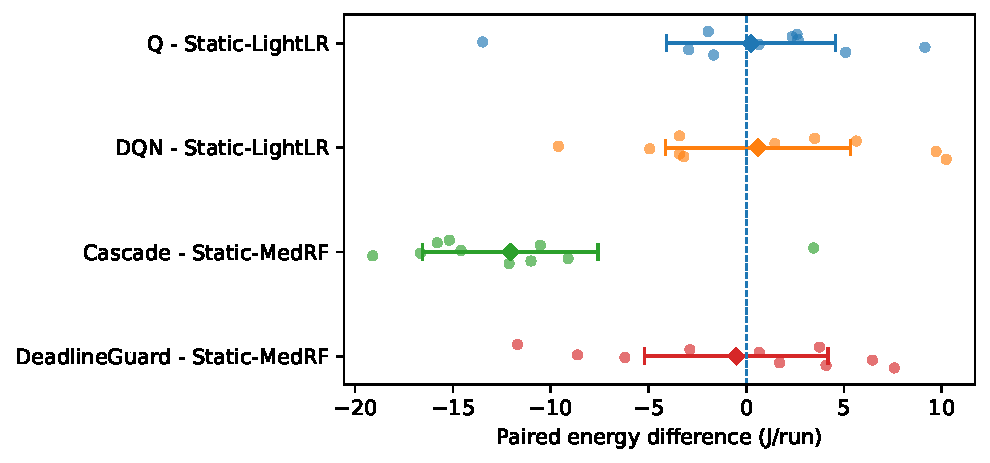
\includegraphics[width=\columnwidth]{figures/paired_energy.pdf}
\caption{Block-level energy differences. Points are paired runs; the larger markers and bars show means and nominal 95\% Student-$t$ intervals. Negative values favor the first method in energy only.}
\label{fig:energy}
\end{figure}

\subsection{Recovery and Idle-Adjustment Sensitivity}
\begin{table*}[t]\centering\footnotesize
\caption{Energy sensitivities, in J/run. Each entry is mean difference [nominal paired 95\% CI]. A: all ten blocks; B: exclude block 1; C: exclude blocks 1 and 5. Adjusted energy subtracts the corresponding preceding-idle baseline.}\label{tab:sensitivity}
\setlength{\tabcolsep}{4pt}\begin{tabular}{llrrr}\toprule Contrast & Endpoint & A ($n=10$) & B ($n=9$) & C ($n=8$)\\\midrule
Q--LR & Raw & $+0.25\;[-4.05,4.55]$ & $+0.49\;[-4.37,5.35]$ & $+2.23\;[-0.93,5.40]$\\
Q--LR & Adjusted & $-4.79\;[-17.15,7.56]$ & $-2.69\;[-15.69,10.31]$ & $+1.59\;[-8.22,11.41]$\\
DQN--LR & Raw & $+0.60\;[-4.12,5.32]$ & $+1.05\;[-4.21,6.30]$ & $+2.38\;[-2.58,7.33]$\\
DQN--LR & Adjusted & $+0.97\;[-9.67,11.62]$ & $+2.12\;[-9.65,13.88]$ & $+3.77\;[-9.16,16.71]$\\
C--RF & Raw & $-12.06\;[-16.55,-7.58]$ & $-11.72\;[-16.75,-6.69]$ & $-11.36\;[-17.13,-5.59]$\\
C--RF & Adjusted & $-16.09\;[-26.72,-5.46]$ & $-16.41\;[-28.50,-4.33]$ & $-14.86\;[-28.29,-1.44]$\\
DG--RF & Raw & $-0.52\;[-5.21,4.18]$ & $+0.73\;[-3.57,5.02]$ & $+1.89\;[-1.99,5.78]$\\
DG--RF & Adjusted & $+3.09\;[-4.91,11.10]$ & $+4.06\;[-4.73,12.84]$ & $+6.56\;[-1.14,14.26]$\\
\bottomrule\end{tabular}\end{table*}

The Q--LR and DQN--LR intervals span zero in every analysis set, with and without idle adjustment. The Cascade--RF mean remains negative across all six combinations. Its raw estimate changes from $-12.06$ J in A to $-11.36$ J in C; the idle-adjusted estimate changes from $-16.09$ J to $-14.86$ J. DeadlineGuard--RF is unresolved in all combinations: the raw means are $-0.52$, $+0.73$, and $+1.89$ J in A, B, and C, respectively.

The wider adjusted intervals show that preceding-idle subtraction introduces its own baseline uncertainty. Agreement in the sign of the cascade contrast under these analyses supports its direction within this dataset and runtime, but does not prove that temporal or instrumentation effects have been eliminated.

\section{Discussion and Limitations}\label{sec:discussion}
\subsection{What Counts as Adaptation?}
A selector can be useful by changing detectors across windows, by escalating selected rows within a batch, or by enforcing a service constraint. Those mechanisms require different evidence. Action occupancy distinguishes the first from a fixed operating point. Cascade branch execution tests the second. Deadline and backlog outcomes test the third. In this experiment, only the cascade implements input-dependent escalation; the learned selectors and DeadlineGuard remain on fixed detectors.

The matched static comparison is consequently essential. Energy savings against a heavier detector can be explained by model choice even when a policy is complicated to train or deploy. Conversely, an unresolved RL--static energy contrast should not be converted into a precise controller-only joule cost. Whole-board measurement includes the complete runtime and is reported at that boundary.

\subsection{Objective and Information Boundaries}
The reward assigns a service penalty, but the training surrogate never develops carryover. A penalty that never activates cannot teach recovery from congestion. Temperature is safety telemetry only. These facts restrict the demonstrated capability even though the implementation can encode queue states and stop unsafe physical runs.

Cascade observes current-row LightLR scores after entry inference; pre-window RL does not. The comparison is therefore between implemented selection mechanisms with their respective information costs, not an ablation in which only the learning rule changes. Likewise, fixed power profiles are optimization proxies, while the reported energy is contemporaneous physical measurement. The preference condition in Section~\ref{sec:preference} helps inspect this proxy objective, not equate it with the measured service outcome.

\subsection{Scope}
The physical results concern one Pi, one power meter, fixed classifiers, and TON-IoT feature replay. They exclude capture, feature extraction, training energy, and multi-node coordination. The detector seed is fixed; block variability does not include variation across independently retrained classifiers, sites, or hardware units. Auxiliary CICIoT2023 and N-BaIoT classification results in the supplement do not establish cross-dataset power generalization.

The test pool had been examined before the current design. Policy selection uses validation only, but this history limits claims of untouched-test generalization. The resampled workloads change arrival counts and prevalence, not the underlying attack families. All methods finish within the tested service budget, so overload and a switching-optimal regime remain outside the demonstrated operating range.

The meter has no independent laboratory calibration or ambient-temperature logger. Blocks 1 and 5 cross recovery periods, and monitoring cadence changes before the later recovery. Exclusion and idle-adjustment analyses quantify sensitivity without removing every possible confound. Nominal intervals are conditional on these runs and should not be read as fleet-level uncertainty.

\section{Conclusion}\label{sec:conclusion}
We compared static, learned, deadline-based, and confidence-driven detector selection using ten paired physical blocks. Q-learning and DQN selected LightLR throughout and offered no resolved energy improvement over direct deployment of that detector. DeadlineGuard remained on MedRF, and every method met the recorded deadlines. The confidence cascade reduced energy relative to MedRF while making a small but measurable detection trade-off. These results favor evaluating selection at its actual information and measurement boundary: compare with the realized static detector, report both security and service outcomes, and inspect whether the objective and training support permit meaningful changes in action.

\section*{Code and Data}
Code, configurations, run summaries, and table-reproduction scripts are available at \url{https://github.com/Nuonan-Ouyang-PhD/tnsm-energy-aware-ids}. The supplementary material reports complete paired comparisons and dataset-specific preparation details.
\bibliographystyle{IEEEtran}\bibliography{references}
\end{document}
